\phantom{I}
\vspace{3cm}
\section{Supplementary results}
%%
This appendix supplements the results section for the materials not shown in the main text. It provides  phonon dispersions computed and electron-hole coupling coefficients and optical spectra as obtained from the solution of the Bethe-Salpeter equation. 


\subsection{Computational details}\label{app_comp_details}
The numerical results presented in this thesis are obtained with two different codes: The pseudopotential code \textsc{Q\!u\!a\!n\!t\!u\!m} ESPRESSO\cite{quantumespresso} and the full-potential all-electron code \exciting{}\cite{exciting}. In the following, it is summarized which code is used for which calculation, and the computational parameters are presented. The various grids for $\k$ and $\q$-points are given in Table~\ref{grids}. \par

\textsc{Q\!u\!a\!n\!t\!u\!m} ESPRESSO is used for all systems to relax the crystal structure and to calculate the phonon modes as well as the Born effective charges. The ground-state  DFT calculations are performed within the general gradient approximation (GGA) using the PBEsol functional\cite{pbesol}. The LO-TO splitting is computed including the nonanalytical part of the force constants  (see (Eq.\;\eqref{forceconst_an}) through the Born effective charges and the high-frequency dielectric tensor.\par
Ground-state calculations also performed with \exciting{}, followed by the study of excitonic properties  through the solution of the BSE. The basis size is set by the parameter $R_\text{MT}|\mathbf{G+k}|_\text{max} = 7.0$, which is found to be sufficient for converging the ground-state total energy of all systems. For the computation of spectra, the grids are shifted by  ($0.097/N_x$, $0.273/N_y$, $0.493/N_z$) (in lattice coordinates), in order to break the symmetry.  For computing binding energies, however, unshifted grids are used such to include the $\Gamma$-point. This is relevant as, in these materials, the electron-hole coupling coefficients of the lowest-energy excitation are largest at this point. Local-field effects are included up to a cutoff of $|\mathbf{G+q}|_\text{max}=3.0\,\text{a.u.}^{-1}$, and 100 empty states are used in the RPA screening. A scissor operator is used in the screening and the BSE part to adjust the computed band gaps to the experimental values from Table~\ref{table_dynscreen}. In the calculation of optical spectra, four valence bands and five conduction bands are considered, and a broadening of 0.3\,eV is applied. For the computation of the excitonic binding energy, three valence and two conduction bands are included (for LiF, five valence and four conduction bands).\par
%
\begin{table}[t]
\captionsetup{format=plain}
\caption[Grids for $\k$ and $\q$-points employed in the different calculations.]{Grids for $\k$ and $\q$-points employed in the different calculations: Ground state (GS), BSE (for MgO, different grids are used for the calculation of the optical spectrum and the binding energy $E^{\phantom{el}}_\text{B}$), and phonons.\label{grids}}
\vspace{1mm}
   \begin{tabularx}{\textwidth}{YYYY}
    \hline
    \hline
    Material  & $\k$-grid (GS) & $\k$-grid (BSE) & $\q$-grid (phonons) \\
    \hline
    LiF  & 10$\times$10$\times$10 & 12$\times$12$\times$12 & 4$\times$4$\times$4  \\
    MgO   &  10$\times$10$\times$10  & 12$\times$12$\times$12 (spec.) & 4$\times$4$\times$4\\
           &  & 18$\times$18$\times$18 ($E^{\phantom{el}}_\text{B}$) & \\
    ZnS  &  10$\times$10$\times$10  & 12$\times$12$\times$12 & 4$\times$4$\times$4\\
    GaN  &  10$\times$10$\times$8 & 12$\times$12$\times$8 & 4$\times$4$\times$4\\
    ZnO  &  10$\times$10$\times$8 & 12$\times$12$\times$8 & 4$\times$4$\times$4\\
    \hline
    \hline
    \end{tabularx}
\end{table}

\newpage

\subsection{Structure relaxation}
The following Table~\ref{tab_struct} summarizes the relaxed structure constants found for the different materials. 
\begin{table}[h]
\captionsetup{format=plain}
    \caption[Relaxed structure constants of the investigated materials in bohr.]{Relaxed structure constants $a$ in bohr of the investigated materials as computed and found by experiment. For GaN and ZnO in the wurtzite structure, the ratios $c/a$ are shown as well. Experimental values for LiF from\cite{lif_lattice}, for MgO from\cite{mgo_lattice}, for ZnS from\cite{zns_lattice}, for GaN from\cite{gan_lattice}, and for ZnO from\cite{zno_lattice}. }
    \vspace{1mm}
   \begin{tabularx}{\textwidth}{YYYYY}
    \hline
    \hline
     Material & $a$   & $c/a$  & $a$ (Expt.) & $c/a$ (Expt.)\\
     \hline
    LiF &  7.68 & -   & 7.61 & - \\
    MgO &  7.97 & -   &   8.03 & -  \\
    ZnS & 10.12 & -   &    10.22 & - \\
    GaN & 6.02 & 1.63  &   6.03 &  1.63   \\
    ZnO & 6.10 & 1.61 &   6.15 & 1.60   \\
    \hline
    \hline
    \end{tabularx}
    \label{tab_struct}
\end{table} 

\newpage
\subsection{Phonon dispersions}\label{app_phonon}

Figure~\ref{phonon_appendix} shows the computed phonon dispersions of ZnS, GaN, and ZnO along high-symmetry directions in the Brilouin zone.
\begin{figure}[H]
\centering
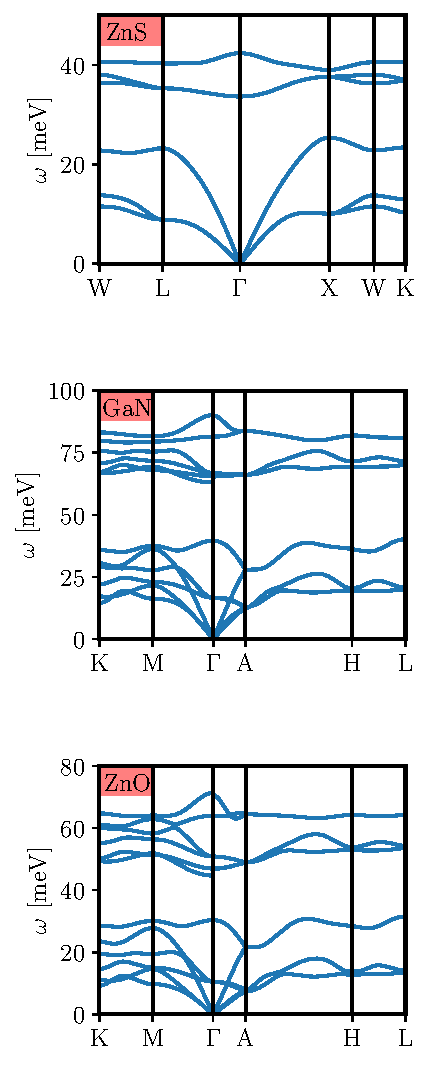
\includegraphics{work/plots/phonons/phonons_app.pdf}

\caption[ Phonon-dispersion curves of ZnS, GaN and ZnO.]{ Phonon-dispersion curves of ZnS (upper panel), GaN (middle panel), and ZnO (lower panel) along high-symmetry directions in the Brillouin zone. \label{phonon_appendix}}

\end{figure}

\subsection{Optical spectra}\label{app_excana}

\begin{figure}[H]

  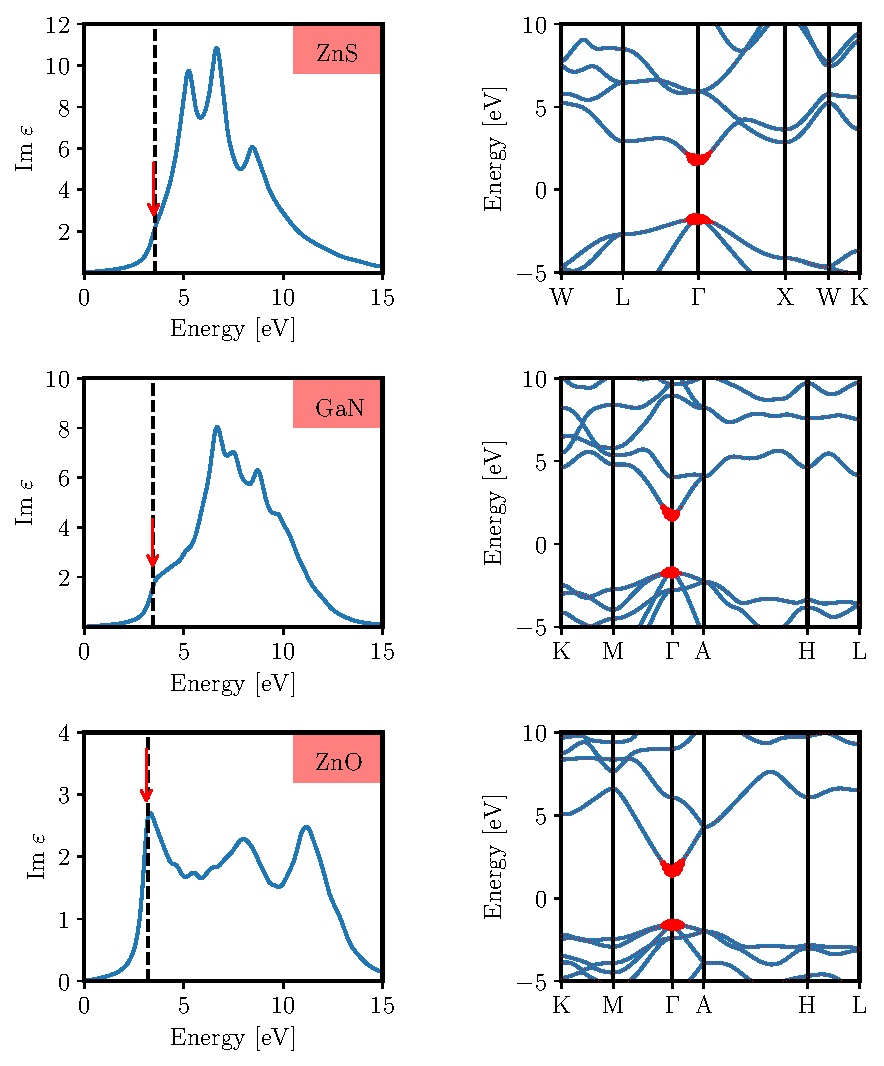
\includegraphics{work/plots/spectra/spectrum_zns_gan_zno.pdf}%
  \caption[Optical spectrum for ZnS, GaN and ZnO.]{Optical spectrum (left) and e-h coupling coefficients of the first exciton (right) of ZnS (upper panel), GaN (middle panel), and ZnO (lower panel). For  GaN and ZnO in the wurtzite structure, the spectra correspond to  light polarized perpendicular to the crystallographic $c$ direction. The position of the first exciton is marked by a red arrow. \label{spectrum_appendix}}
\end{figure}


\newpage
\subsection{Experimental values}

In Table~\ref{tab_exp_data}, we show the experimental values for the elements of the Born-effective charge tensor $\mathbf{Z}^*$, the full static dielectric tensor $\boldsymbol{\varepsilon}_0$, and the highest LO phonon frequencies.

\begin{table}[h]
\captionsetup{format=plain}
\caption[Experimental parameters relevant for EPI.]{Experimental parameters: Elements of the full static dielectric tensor  $\boldsymbol{\varepsilon}_0$ and the Born-effective charge tensor $\mathbf{Z}^*$, and the highest LO frequency in\,meV. Only non-vanishing tensor elements are shown, parallel and perpendicular ($\parallel,\perp$) are to be understood with respect to the $\mathbf{c}$-axis of the wurtzite crystals.  Data for LiF from \cite{lif_charges,lif_tensor,lif_phonon}, for MgO from \cite{mgo_charges,mgo_data}, for ZnS  from \cite{zns_charges,bechstedt2016many}, for ZnO from \cite{zno_data}, and for GaN from \cite{gan_data,gan_charges,gan_tensor}.\label{tab_exp_data}}
\vspace{1mm}
   \begin{tabularx}{\textwidth}{YYYY}
    \hline
    \hline
    Material  & $\boldsymbol{\varepsilon}_0$ & $\omega^{\phantom{I}}_\text{LO}$ [meV] & $|\mathbf{Z}^*|$ [a.u.] \\
    \hline
    LiF  & 9.0 & 82  &  1.0 \\
    MgO  & 9.8 & 89  & 2.0 \\
    ZnS  & 8.3  & 37  & 2.2 \\
    GaN  &  9.5($\perp$), 10.4 ($\parallel$)  & 91  &  2.7($\perp$), 2.8 ($\parallel$) \\
    ZnO  & 7.8($\perp$), 8.9 ($\parallel$)  & 73  & 2.1 ($\perp$), 2.1($\parallel$)\\
    \hline
    \hline
    \end{tabularx}
\end{table}


\newpage

\phantom{.}
\vspace{3cm}
\section{Periodic crystals}\label{bloch_waves}
%------------
%------------
In this appendix, the description of a periodic solid and the properties of Bloch waves in a periodic potential are reviewed. Furthermore, some useful integrals and summations over the crystal lattice are summarized.

%------------
\subsection{Crystal lattice}
%------------

Consider an infinite crystal composed of periodically arranged atoms. The crystal structure is described by a periodically repeated unit cell having the volume $\Omega^{\phantom{I}}_\text{UC}$, which is defined by a set of three basis vectors $\{\mathbf{a}_1,\mathbf{a}_2,\mathbf{a}_3\}$. All integer combination of the basis vectors  define the set of lattice vectors $\{\mathbf{R}\}$. For the theoretical study of crystals, the definition of a reciprocal lattice is useful. The basis vectors $\{\mathbf{b}_1,\mathbf{b}_2,\mathbf{b}_3\}$ in reciprocal space are defined by
%
\begin{equation}
    \mathbf{a}_i\cdot\mathbf{b}_j = 2\pi\,\delta_{ij} \quad   \forall \; i,j \in \{1,2,3\}.
\end{equation}
%
Accordingly, the set of reciprocal lattice vectors  $\{\mathbf{G}\}$ is given by all integer combinations of the reciprocal basis vectors.\par
Usually, just a finite number of unit cells $N_p=N_x\!\times\!N_y\!\times\!N_z$ is considered instead of infinitely large crystals. The set of these unit cells define the Born-von-K\'{a}rm\'{a}n (BvK) volume $V$=$N_p\,\Omega^{\phantom{I}}_\text{UC}$.\newpage
\noindent Commonly used identities over the BvK volume involving the lattice vectors are  given in the following:
%
\begin{align}
    \frac{1}{V}\int_V \text{\!\!d}\mathbf{r}\,e^{i\mathbf{(q-q')\cdot r}} & = \delta_\mathbf{qq'},\\[10pt]
    \frac{1}{N_p}\sum_\mathbf{R}e^{i\mathbf{(q-q')\cdot r}}  & = \delta_\mathbf{qq'}\label{crystalsum}.
\end{align}

%------------
\subsection{Bloch waves}
%------------
In a periodic potential obeying $v(\mathbf{r+R})=v(\mathbf{r})$ for any lattice vector $\mathbf{R}$, Bloch's theorem states that the solutions of the Schr\"odinger equation are of the form 
%
\begin{align}\label{bloch_int}
    \psi_{n\mathbf{k}}(\mathbf{r}) =  u_{n\mathbf{k}}(\mathbf{r})\,e^{i\mathbf{k\cdot r}},
\end{align}
%
where $u_{n\mathbf{k}}(\mathbf{r})=u_{n\mathbf{k}}(\mathbf{r+R})$ has the periodicity of the lattice. Bloch waves are labeled by a band index $n$ and a wave-vector $\mathbf{k}$. Not only electronic wavefunctions, but also other quantites may have a Bloch form, for instance the electron-phonon coupling function can be written as
%
\begin{equation}\label{blochcoupl2}
        g_{\mathbf{q}\nu}(\mathbf{r}) = e^{i\mathbf{q\cdot r}}\,\Delta_\text{P}^{\!\mathbf{q}\nu}v      ^{\phantom{I}}_\text{KS}(\mathbf{r}),
\end{equation}
%
where $\Delta_\text{P}^{\!\mathbf{q}\nu}v      ^{\phantom{I}}_\text{KS}(\mathbf{r})$ is the cell-periodic part of the function. In the main text, the Fourier coefficient of the coupling function is needed which is defined according to Eq.\;\eqref{fourier_coeff1}~as
%
\begin{align}\label{coupling_fourier2}
     \Tilde{g}_{\mathbf{q'}\nu}^{\mathbf{G}}(\mathbf{q}) = \frac{1}{V} \int \text{\!\!d}^3\mathbf{r}\, g_{\mathbf{q'}\nu}(\mathbf{r})\,e^{-i(\mathbf{q}+\mathbf{G})\cdot\mathbf{r}}.
\end{align}
%
Formally, the integration is to be taken over the whole crystal volume $V$, but due to the Bloch-property of the coupling function it can be rewritten as an integral over the unit cell with volume $\Omega^{\phantom{I}}_\text{UC}$. Further, the coefficient is only non-vanishing if $\mathbf{q=q'}$. Considering the Born-von-K\'{a}rm\'{a}n volume, the coordinate of an arbitrary vector $\mathbf{r}$ can \newpage be expressed as the sum of a vector from the unit cell and the coordinate $\mathbf{R}_p$ of the $p$th unit cell. The integral can accordingly be rewritten as
%
\begin{equation}\label{blochdelta}
    \begin{aligned}
    \frac{1}{V} \int_V \text{\!\!d}^3\mathbf{r}\, g_{\mathbf{q'}\nu}(\mathbf{r})\,e^{-i(\mathbf{q}+\mathbf{G})\cdot\mathbf{r}} & =  \frac{1}{V} \int_V \text{\!\!d}^3\mathbf{r}\,\Delta_\text{P}^{\!\mathbf{q}\nu}v      ^{\phantom{I}}_\text{KS}(\mathbf{r})\,e^{-i(\mathbf{q-q'+G)\cdot r}}\\[10pt]
     & = \frac{1}{V} \sum_p\int_{\Omega^{\phantom{I}}_\text{UC}} \text{\!\!d}^3\mathbf{r}\,\Delta_\text{P}^{\!\mathbf{q}\nu}v      ^{\phantom{I}}_\text{KS}(\mathbf{r})\,e^{-i(\mathbf{q-q'+G})\cdot(\mathbf{r}+\mathbf{R}_p)}\\[10pt]
     & = \frac{1}{V} \sum_p e^{-i(\mathbf{q-q'+G})\cdot\mathbf{R}_p}\\[10pt] 
     & \phantom{iiiiiiii} \times \int_{\Omega^{\phantom{I}}_\text{UC}}\text{\!\!d}^3\mathbf{r}\,\Delta_\text{P}^{\!\mathbf{q}\nu}v      ^{\phantom{I}}_\text{KS}(\mathbf{r})\,e^{-i\mathbf{(q-q'+G)\cdot r}}\\[10pt]
     & =  \delta_\mathbf{qq'}\frac{1}{\Omega^{\phantom{I}}_\text{UC}} \int_{\Omega^{\phantom{I}}_\text{UC}} \text{\!\!d}^3\mathbf{r}\, g_{\mathbf{q'}\nu}(\mathbf{r})\,e^{-i(\mathbf{q}+\mathbf{G})\cdot\mathbf{r}}.
    \end{aligned}
\end{equation}
%
In the last equality, the result of the crystal summation in Eq.\;\eqref{crystalsum} was used.


\newpage

\phantom{.}
\vspace{3cm}
\section{Mathematical tools}

\subsection{Fourier transformations}
Here, we summarize the conventions used in the thesis for various Fourier transformations. The expressions are given without proof, they can be found in any book in solid-state theory. 

\subsubsection{Functions in time}\label{fourier_time}

Any function in the time domain $f(t)$ can be transformed into the frequency domain~by
%
\begin{align}
       F(\omega) = \int\text{\!\!d}t\,f(t)\,e^{i\omega t}.
\end{align}                                          
%
The inverse transformation is given by
%
\begin{align}
    f(t) = \frac{1}{2\pi}\int\text{\!\!d}\omega\,F(\omega)\,e^{-i\omega t}.
\end{align}

\newpage

\subsubsection{Functions in real space}
%
Any function in real space $f(\mathbf{r})$   can be represented in terms of its Fourier components $F_\mathbf{G}(\mathbf{q})$ as 
%
\begin{align}\label{fourier_real_onearg}
    f(\mathbf{r}) = \sum^\text{BZ}_\mathbf{q}\sum_\mathbf{G}F_\mathbf{G}(\mathbf{q})\,e^{i\mathbf{(q+G)\cdot r}},
\end{align}
%
where the coefficients of the expansion are given by
%
\begin{align}\label{fourier_coeff1}
    F_\mathbf{G}(\mathbf{q}) = \frac{1}{V}\int_V \text{\!\!d}\mathbf{r}\,f(\mathbf{r})\,e^{-i\mathbf{(q+G)\cdot r}}.
\end{align}
%
The integration extends over the Born-von-K\'{a}rm\'{a}n (BvK) volume $V$. Equivalently, any function depending $f(\mathbf{r,r'})$ on two spatial coordinates can be given by its Fourier representation as
%
\begin{align}
    f(\mathbf{r,r'}) = \frac{1}{V}\sum^\text{BZ}_\mathbf{q,q'}\sum_\mathbf{G,G'}\,e^{i\mathbf{(q+G)\cdot r}}F_\mathbf{G,G'}(\mathbf{q,q'})\,e^{-i\mathbf{(q'+G')\cdot r'}}
\end{align}
%
and the Fourier coefficients are defined as
%
\begin{align}\label{fourier_coeff}
      F_\mathbf{G,G'}(\mathbf{q,q'}) = \frac{1}{V}\int\!\!\int_V \text{\!\!d}\mathbf{r}\text{d}\mathbf{r'}\,e^{-i\mathbf{(q+G)\cdot r}}\,f(\mathbf{r,r'})\,e^{i\mathbf{(q'+G')\cdot r'}}.
\end{align}



%-----------------
\subsubsection{Periodic functions}
%-----------------
In the case of a lattice periodic function  in a periodic crystal depending on one spatial argument, \textit{i.e.} $f(\mathbf{r+R})=f(\mathbf{r})$, only the coefficient corresponding to $\mathbf{q}=0$ will give a contribution to the expansion, such that in this case
%
\begin{align}
    f(\mathbf{r}) = \sum_\mathbf{G}F_\mathbf{G}(0)\,e^{-i\mathbf{G\cdot r}}.
\end{align}
%
Similarly, if a function of two coordinates in real space is periodic with respect to a shift of both arguments by the same lattice vector, \textit{i.e.}, $f(\mathbf{r+R,r'+R})=f(\mathbf{r,r'})$, the Fourier coefficients will only depend on one single reciprocal coordinate and the representation is given by
%
\begin{equation}\label{fourier_periodic}
     f(\mathbf{r,r'}) = \frac{1}{V}\sum^\text{BZ}_\mathbf{q}\sum_\mathbf{GG'}\,e^{i\mathbf{(q+G)\cdot r}}\,F_\mathbf{GG'}(\mathbf{q})\,e^{-i\mathbf{(q+G')\cdot r'}}.
\end{equation}
%
\newpage
\noindent The Fourier coefficients are obtained by integrating over the BvK volume $V$ according~to

%
\begin{align}\label{fourier_coeff_periodic}
      F_\mathbf{GG'}(\mathbf{q}) = \frac{1}{V}\int_V \text{\!\!d}\mathbf{r}\text{d}\mathbf{r'}\,e^{-i\mathbf{(q+G)\cdot r}}\,f(\mathbf{r,r'})\,e^{i\mathbf{(q+G')\cdot r'}}.
\end{align}


\subsection{Residue theorem}\label{residue}
Consider a positively oriented simple closed contour $C$ in the complex plane and a function $f(z)$ of a complex variable $z$ having $n$ poles inside the contour. The residue theorem states that integral over this contour can be evaluated by 
%
\begin{align}
    \int_C \text{\!\!d}z\,f(z) = 2\pi\,i\,\sum_k \underset{z=a_k}{\text{Res}}\,f(z),
\end{align}
%
where $\underset{z=a_k}{\text{Res}}\,f(z)$ is the residue of $f$ with respect to the pole $k$. The residue of a simple pole can be obtained according to
%
\begin{equation}\label{residue_pole}
   \underset{z=a_k}{\text{Res}}\,f(z) = \lim_{z\rightarrow a_k}(z-a_k)\,f(z).
\end{equation}

% A special application of the residue theorem is an integral along the real axis, as shown in Fig.~\ref{residue}. If possible, the contour is in this case chosen such that any additional contribution which is not on the real axis vanishes. In many cases, this is possible as the integrand decays exponentially in the upper or the lower half of the complex plane. Then, only the residues of the poles in the upper or lower half contribute to the integral.


%  \begin{figure}[H]
% \centering
% \begin{tikzpicture}[node distance=8cm]
% \node (xstart) {};
% \node (xend) [right of=xstart] {Re $z$};
% \node (ystart) [below of=xstart, xshift = 4 cm, yshift =  + 5cm] {};
% \node (yend) [above of=ystart,yshift=-2cm] {Im $z$};
% \node (center)[above of=ystart,xshift=3cm,yshift=-5cm] {};



% \node (a1) [above of =xstart, xshift = 2cm,yshift = -8.5cm,  circle,fill,inner sep=1.5pt]{};
% \node (texta1) [above of =xstart, xshift = 2cm,yshift = -9cm]{$a_1$};
% \node (a2) [above of =xstart, xshift = 3cm,yshift = -8.5cm,  circle,fill,inner sep=1.5pt]{};
% \node (texta2) [above of =xstart, xshift = 3cm,yshift = -9cm]{$a_2$};
% \node (a3) [above of =xstart, xshift = 5cm,yshift = -8.5cm,  circle,fill,inner sep=1.5pt]{};
% \node (texta3) [above of =xstart, xshift = 5cm,yshift = -9cm]{$a_n$};

% \node (b1) [above of =xstart, xshift = 3cm,yshift = -7.5cm,  circle,fill,inner sep=1.5pt]{};
% \node (textb1) [above of =xstart, xshift = 3cm,yshift = -7cm]{$b_1$};
% \node (b2) [above of =xstart, xshift = 4.5cm,yshift = -7.5cm,  circle,fill,inner sep=1.5pt]{};
% \node (textb2) [above of =xstart, xshift = 4.5cm,yshift = -7cm]{$b_2$};
% \node (b3) [above of =xstart, xshift = 6.5cm,yshift = -7.5cm,  circle,fill,inner sep=1.5pt]{};
% \node (textb3) [above of =xstart, xshift = 6.5cm,yshift = -7cm]{$b_{m}$};
% \node (textb3) [above of =xstart, xshift = 6.5cm,yshift = -10cm]{$C$};

% \node (dots1) [above of =xstart, xshift = 4.3cm,yshift = -8.5cm]{...};
% \node (dots2) [above of =xstart, xshift = 5.5cm,yshift = -7.5cm]{...};
% \node (linepoint) [above of =xstart, xshift = 5.5cm,yshift = -8cm]{};



% \draw  [->,>=stealth',very thick]   (xstart) -- (linepoint.center) ;
% \draw [line]   (linepoint.center) -- (xend) ;
% \draw [line]   (ystart) -- (yend) ;
% \draw [->,>=stealth',very thick] (center) arc (-10:-170:3cm);
% \end{tikzpicture}

% \caption{\label{residue} An integral along the real axis is expressed as a contour integral.}
% \end{figure}



%------------
%------------




